\documentclass[12pt,a4paper]{report}

\usepackage[utf8]{inputenc}
\usepackage[a4paper, top=1in, bottom=1in, right=1in, left=1.25in]{geometry}
\usepackage{mathptmx} % Times New Roman font equivalent
\usepackage{setspace}
\setstretch{1.5} % 1.5 line spacing as required
\usepackage{amsmath,amssymb}
\usepackage{graphicx}
\usepackage{booktabs}
\usepackage{tabularx}
\usepackage{titlesec}
\usepackage{fancyhdr}
\usepackage[font={bf,normalsize},labelfont=bf,justification=centering]{caption}
\usepackage{hyperref}
\usepackage{tikz}
\usetikzlibrary{shapes.geometric,arrows.meta,positioning,calc}

% Justified text alignment
\hyphenpenalty=1000
\tolerance=2000
\emergencystretch=10pt

% Header and Footer Styling (Page number at bottom center)
\pagestyle{fancy}
\fancyhf{}
\fancyfoot[C]{\thepage}
\renewcommand{\headrulewidth}{0pt}
\renewcommand{\footrulewidth}{0pt}

% Section Headings Styling according to university standards:
% Chapter / Main Title: 16pt Bold
% Section Heading: 14pt Bold
% Sub-section Heading: 12pt Bold
\titleformat{\chapter}[display]
  {\normalfont\fontsize{16}{20}\bfseries\centering}{\chaptertitlename\ \thechapter}{10pt}{\fontsize{16}{20}\bfseries}
\titlespacing*{\chapter}{0pt}{-10pt}{20pt}

\titleformat{\section}
  {\normalfont\fontsize{14}{18}\bfseries}{\thesection}{1em}{}
\titlespacing*{\section}{0pt}{14pt}{6pt}

\titleformat{\subsection}
  {\normalfont\fontsize{12}{15}\bfseries}{\thesubsection}{1em}{}
\titlespacing*{\subsection}{0pt}{10pt}{4pt}

\titleformat{\subsubsection}
  {\normalfont\fontsize{12}{15}\bfseries}{\thesubsubsection}{1em}{}
\titlespacing*{\subsubsection}{0pt}{8pt}{3pt}

\hypersetup{
    colorlinks=true,
    linkcolor=black,
    citecolor=black,
    urlcolor=blue
}

\begin{document}

% ==============================================================================
% TITLE PAGE
% ==============================================================================
\begin{titlepage}
    \centering
    \vspace*{0.5cm}
    
    {\fontsize{16}{22}\bfseries A PROJECT PROPOSAL\par}
    \vspace{0.6cm}
    {\fontsize{14}{18}\bfseries ON\par}
    \vspace{0.6cm}
    {\fontsize{16}{22}\bfseries FILE COMPRESSION SYSTEM USING HUFFMAN CODING\par}
    \vspace{2.0cm}
    
    {\fontsize{12}{16}\selectfont A Project Proposal Submitted in Partial Fulfillment of the\\
    Requirements for the Degree of Bachelor of Technology\par}
    \vspace{3.0cm}
    
    \begin{minipage}{0.45\textwidth}
        \begin{flushleft}
            {\fontsize{12}{15}\bfseries Submitted By:}\\[0.3cm]
            {\fontsize{12}{15}\bfseries Aarti Kushwaha}
        \end{flushleft}
    \end{minipage}
    \hfill
    \begin{minipage}{0.45\textwidth}
        \begin{flushright}
            {\fontsize{12}{15}\bfseries Under the Guidance of:}\\[0.3cm]
            {\fontsize{12}{15}\bfseries Project Supervisor}
        \end{flushright}
    \end{minipage}
    
    \vfill
    {\fontsize{12}{15}\bfseries Academic Session 2025--2026\par}
\end{titlepage}

% ==============================================================================
% PRELIMINARY PAGES (ROMAN NUMERALS)
% ==============================================================================
\pagenumbering{roman}
\setcounter{page}{1}

% Certificate / Approval Page
\chapter*{Certificate of Approval}
\thispagestyle{fancy}

This is to certify that the project proposal entitled \textbf{``File Compression System Using Huffman Coding''} submitted by \textbf{Aarti Kushwaha} in partial fulfillment of the requirements for the award of the Degree of Bachelor of Technology has been examined and approved as an authentic proposal work carried out under supervision.

\vspace{3.0cm}
\noindent
\begin{minipage}{0.45\textwidth}
    \hrulefill\\
    \centering
    \textbf{Project Supervisor}
\end{minipage}
\hfill
\begin{minipage}{0.45\textwidth}
    \hrulefill\\
    \centering
    \textbf{Internal / External Examiner}
\end{minipage}

\newpage
\tableofcontents
\newpage

% ==============================================================================
% CHAPTER 1: PROJECT PROPOSAL BODY (NUMERIC PAGE NUMBERING FROM 1)
% ==============================================================================
\pagenumbering{arabic}
\setcounter{page}{1}

\chapter{Introduction}

\section{Introduction}
In modern computing environments, the rapid expansion of digital information has made efficient data transmission and compact storage critical necessities. Data compression algorithms minimize the physical space required to store information while conserving transmission bandwidth across communications networks.

Compression methods are fundamentally categorized into lossy and lossless algorithms. While lossy compression achieves higher compression ratios by discarding perceptual redundancies (such as in audio or photographic formats), lossless compression reconstructs original binary data exactly, bit-for-bit. For text documents, source code, database dumps, and application binaries, lossless compression is strictly mandatory.

This project focuses on the study, design, and implementation of a \textbf{File Compression System} using the classical \textbf{Huffman Coding algorithm}. The application enables users to compress and decompress arbitrary files efficiently through an interactive web-based graphical interface with complete lossless integrity.

\section{Background Study}
The theoretical foundation of lossless compression originated in Claude Shannon's landmark 1948 paper, \textit{``A Mathematical Theory of Communication''}, which defined the concept of Shannon Entropy as the fundamental lower bound on the average number of bits required to encode symbol alphabets. 

In 1952, David A. Huffman developed an optimal greedy method for constructing variable-length prefix-free codes based on known symbol occurrence frequencies. Huffman coding establishes an optimal prefix property: no assigned code string is a prefix of any other code string, allowing continuous and unambiguous sequential decoding without special delimiters. 

In conventional computing environments, proprietary or complex compression utilities often mask the underlying algorithmic mechanisms. This proposal aims to provide an accessible, self-contained implementation that bridges theoretical information theory with practical software engineering.

\section{Scope}
The scope of this project encompasses:
\begin{enumerate}
    \item Development of an automated byte-frequency counter and min-heap binary tree generator in software.
    \item Generation of variable-length prefix codes and bit-level bitstream packing for arbitrary file formats.
    \item Embedding self-contained header metadata containing serialized tree structures to permit independent decompression.
    \item Lossless decompression engine to restore encoded files byte-for-byte with SHA-256 verification.
    \item A clean, responsive user interface allowing drag-and-drop file upload, compression tracking, and history management.
\end{enumerate}

\section{Limitations}
The system operates under the following identified limitations:
\begin{enumerate}
    \item \textbf{Pre-compressed File Limitations}: Files that already exhibit high Shannon entropy (such as JPEG images, MP4 videos, or previously compressed ZIP files) cannot be substantially compressed further and may slightly expand due to the overhead of the frequency dictionary header.
    \item \textbf{Static Huffman Tree Overhead}: For very small input files (e.g., files under 100 bytes), the storage cost of transmitting the codebook frequency table in the header can exceed the space saved from bit-level compaction.
    \item \textbf{Single-Node Execution}: Initial implementation is targeted for standalone desktop and local web server execution rather than distributed cloud clusters.
\end{enumerate}

% ==============================================================================
% CHAPTER 2: PROBLEM STATEMENT & OBJECTIVES
% ==============================================================================
\chapter{Problem Statement \& Objectives}

\section{Problem Statement}
Every day, computer users and organizations handle vast volumes of documents, log files, configuration data, and scripts. Storing and transmitting these files in raw uncompressed formats consumes excessive hard drive space and overburdens limited network bandwidth.

Existing industrial compression software tools are frequently closed-source, bundle complex external proprietary dependencies, or function as opaque black boxes that do not expose the internal mechanics of entropy reduction. Furthermore, many educational environments lack simple, transparent, and reproducible platforms for demonstrating variable-length entropy coding directly on actual user files.

Therefore, there is an evident need for an efficient, transparent, and robust File Compression System centered on the Huffman Coding algorithm, capable of providing verified lossless file reconstruction through an accessible interface.

\section{Objectives}
The primary objectives of the proposed project are as follows:
\begin{enumerate}
    \item \textbf{Lossless Compression}: To develop a fully functional Huffman compression engine capable of compressing arbitrary file formats without losing a single byte of data.
    \item \textbf{Accurate Decompression}: To implement an inverse tree-traversal decompression engine that reads bitstreams and perfectly reconstructs original files.
    \item \textbf{Optimal Prefix Encoding}: To utilize a min-heap priority queue for constructing prefix-free binary codes with optimal average codeword length.
    \item \textbf{Integrity Verification}: To compute and verify cryptographic SHA-256 checksums before compression and after decompression to ensure total data fidelity.
    \item \textbf{User-Friendly Interface}: To provide an intuitive web-based interface for drag-and-drop file processing, download management, and session activity tracking.
\end{enumerate}

% ==============================================================================
% CHAPTER 3: METHODOLOGY & SYSTEM DESIGN
% ==============================================================================
\chapter{Methodology}

\section{Requirement Identification}

\subsection{Study of Existing System}
An analysis of existing compression utilities reveals that while standard general-purpose utilities (such as gzip, 7-Zip, or WinRAR) achieve high compression ratios, they combine multi-stage algorithms (such as LZ77 dictionary matching with sliding windows followed by dynamic Huffman trees). This multi-stage pipeline makes debugging and educational comprehension complex. A pure, robust implementation of canonical Huffman coding allows direct analysis of symbol probability distribution and prefix code generation without unnecessary complexity.

\subsection{Literature Review}
\begin{enumerate}
    \item \textbf{Shannon (1948)}: Formulated the mathematical foundation of communication and proved that the entropy $H(X) = -\sum P(x_i) \log_2 P(x_i)$ represents the absolute theoretical limit for lossless data compaction.
    \item \textbf{Huffman (1952)}: Published \textit{``A Method for the Construction of Minimum-Redundancy Codes''}, introducing the bottom-up tree generation algorithm using priority queues that guarantees optimal prefix codes for given character probabilities in $O(n \log n)$ time.
    \item \textbf{Knuth (1985)}: Explored dynamic and static Huffman data structures, demonstrating memory-efficient bit-packing techniques and sequential binary tree traversal mechanisms for digital computers.
\end{enumerate}

\subsection{Requirement Analysis}
\subsubsection{Functional Requirements}
\begin{itemize}
    \item The system shall read input files in binary stream mode to support both ASCII text and arbitrary binary data.
    \item The system shall construct byte-frequency tables across 256 possible byte values ($0\text{x}00$ to $0\text{xFF}$).
    \item The system shall build an optimal binary tree using a priority queue.
    \item The system shall generate variable-length bit codewords and write packed bitstreams.
    \item The system shall include self-contained decoding headers in compressed archives.
    \item The system shall decompress archives and restore files with matching checksums.
\end{itemize}

\subsubsection{Non-Functional Requirements}
\begin{itemize}
    \item \textbf{Reliability}: 100\% lossless reconstruction with zero data corruption.
    \item \textbf{Usability}: Clean, modern, and responsive user interface.
    \item \textbf{Performance}: Rapid execution for common documents and source files.
\end{itemize}

\subsubsection{Hardware \& Software Requirements}
\begin{itemize}
    \item \textbf{Hardware Requirements}: Minimum 2.0 GHz Dual-Core CPU, 4 GB RAM, 500 MB free hard disk space.
    \item \textbf{Software Requirements}: Windows 10/11 or Linux OS, Modern Web Browser (Chrome/Firefox/Edge), PHP 8.2+ runtime environment.
\end{itemize}

\section{Feasibility Study}

\subsection{Technical Feasibility}
The system utilizes modern PHP for backend processing, HTML5/CSS3/JavaScript for frontend presentation, and SQLite/MySQL for file logging. PHP provides native bitwise operators, stream wrappers, and hash libraries. Modern browsers support high-performance drag-and-drop file APIs. Hence, the project is completely technically feasible.

\subsection{Operational Feasibility}
The proposed application requires no specialized client-side software installations. Users interact with the platform through any standard web browser. The workflows for compression and decompression are straightforward, requiring only simple file uploads. Therefore, operational feasibility is high.

\subsection{Economic Feasibility}
The entire software stack comprises free, open-source technologies (PHP, SQLite, standard web specifications). No commercial licensing, proprietary compilers, or dedicated paid server infrastructure is required. The project is economically sound and cost-effective.

\section{High Level Design \& Description of Algorithms}

\subsection{Working Mechanism of Proposed System}
The working mechanism of the file compression and decompression lifecycle is summarized below:
\begin{enumerate}
    \item \textbf{Compression Pipeline}:
    \begin{itemize}
        \item Read raw binary data from uploaded file.
        \item Count frequency of each byte value ($0\text{x}00$ to $0\text{xFF}$).
        \item Insert leaf nodes into a min-heap priority queue sorted by frequency.
        \item Repeatedly extract two nodes with the lowest frequencies, create an internal parent node with their combined frequency, and re-insert into the queue until one root node remains.
        \item Traverse the tree from root to leaf to assign binary prefix codes (left branch = `0', right branch = `1').
        \item Encode the original byte sequence using the generated variable-length bit codes.
        \item Pack bits into 8-bit bytes, prepend the frequency header table, and store the output file (`.shuf').
    \end{itemize}
    \item \textbf{Decompression Pipeline}:
    \begin{itemize}
        \item Parse the frequency table header from the `.shuf` file.
        \item Reconstruct the exact Huffman binary tree.
        \item Read packed bits sequentially and traverse the tree from root until reaching a leaf node.
        \item Emit the corresponding original byte and reset traversal to root for the next bits.
        \item Verify original file size and SHA-256 hash checksum.
    \end{itemize}
\end{enumerate}

\begin{figure}[htbp]
\centering
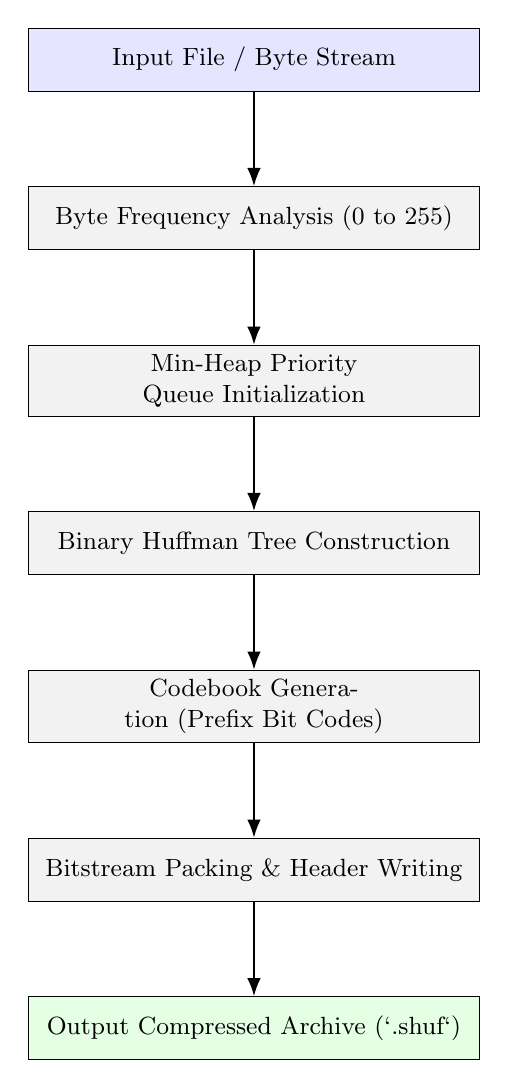
\begin{tikzpicture}[
    node distance=1.2cm and 1.5cm,
    proc/.style={rectangle, draw=black, fill=gray!10, text width=5.5cm, align=center, minimum height=0.8cm, font=\small},
    arrow/.style={-Latex, thick}
]
    \node (in) [proc, fill=blue!10] {Input File / Byte Stream};
    \node (freq) [proc, below=of in] {Byte Frequency Analysis ($0$ to $255$)};
    \node (heap) [proc, below=of freq] {Min-Heap Priority Queue Initialization};
    \node (tree) [proc, below=of heap] {Binary Huffman Tree Construction};
    \node (code) [proc, below=of tree] {Codebook Generation (Prefix Bit Codes)};
    \node (pack) [proc, below=of code] {Bitstream Packing \& Header Writing};
    \node (out) [proc, below=of pack, fill=green!10] {Output Compressed Archive (`.shuf`)};

    \draw [arrow] (in) -- (freq);
    \draw [arrow] (freq) -- (heap);
    \draw [arrow] (heap) -- (tree);
    \draw [arrow] (tree) -- (code);
    \draw [arrow] (code) -- (pack);
    \draw [arrow] (pack) -- (out);
\end{tikzpicture}
\caption{High Level Flowchart of Proposed Huffman Compression System}
\label{fig:flowchart}
\end{figure}

% ==============================================================================
% CHAPTER 4: GANTT CHART & EXPECTED OUTCOMES
% ==============================================================================
\chapter{Project Timeline \& Expected Outcomes}

\section{Gantt Chart (Project Timeline)}
The proposed project is scheduled for a completion timeline of \textbf{four (4) months}. Table~\ref{tab:gantt} illustrates the work breakdown schedule across the four-month implementation lifecycle.

\begin{table}[htbp]
\centering
\caption{Four-Month Project Work Schedule (Gantt Chart)}
\label{tab:gantt}
\begin{tabularx}{\textwidth}{lXXXX}
\toprule
\textbf{Activity / Milestone} & \textbf{Month 1} & \textbf{Month 2} & \textbf{Month 3} & \textbf{Month 4} \\
\midrule
Requirement Gathering \& Feasibility & \textbf{[XXXX]} & & & \\
Literature Review \& Algorithmic Study & \textbf{[XXXX]} & & & \\
System Architecture \& Database Design & & \textbf{[XXXX]} & & \\
Huffman Engine Core Implementation & & \textbf{[XXXX]} & & \\
Bitstream Packing \& Tree Serialization & & & \textbf{[XXXX]} & \\
Web Interface \& API Integration & & & \textbf{[XXXX]} & \\
Lossless Verification \& Testing & & & & \textbf{[XXXX]} \\
Documentation, Report \& Defense & & & & \textbf{[XXXX]} \\
\bottomrule
\end{tabularx}
\end{table}

\section{Expected Outcomes}
Upon completion of this project, the following deliverables and outcomes are anticipated:
\begin{enumerate}
    \item A fully working, lossless file compression and decompression software tool implementing Huffman entropy coding.
    \item Documented size reductions ranging from 20\% to 60\% on text documents, source code, and structured log files.
    \item Perfect file restoration confirmed through automated SHA-256 hash comparison.
    \item An intuitive, web-based graphical interface for effortless drag-and-drop user interaction.
    \item Complete technical documentation and source code repository available for academic evaluation.
\end{enumerate}

% ==============================================================================
% CHAPTER 5: CONCLUSION & REFERENCES
% ==============================================================================
\chapter{Conclusion \& References}

\section{Conclusion}
Data compression continues to serve as an indispensable pillar of modern digital communications and storage architecture. This project proposal establishes the technical blueprint for developing an accessible, reliable, and mathematically verified \textbf{File Compression System} grounded in the principles of \textbf{Huffman Coding}.

By focusing strictly on Huffman entropy encoding, the system eliminates unnecessary complexity while delivering optimal prefix code construction, rigorous lossless restoration, and user-friendly interaction. The planned four-month execution schedule ensures orderly progression from theoretical analysis to full implementation, empirical verification, and academic delivery.

\section{References}
\begin{enumerate}
    \item D. A. Huffman, ``A Method for the Construction of Minimum-Redundancy Codes,'' \textit{Proceedings of the IRE}, vol. 40, no. 9, pp. 1098--1101, Sept. 1952.
    \item C. E. Shannon, ``A Mathematical Theory of Communication,'' \textit{Bell System Technical Journal}, vol. 27, no. 3, pp. 379--423, July 1948.
    \item D. E. Knuth, ``Dynamic Huffman Coding,'' \textit{Journal of Algorithms}, vol. 6, no. 2, pp. 163--180, June 1985.
    \item T. H. Cormen, C. E. Leiserson, R. L. Rivest, and C. Stein, \textit{Introduction to Algorithms}, 3rd ed. Cambridge, MA: MIT Press, 2009.
    \item K. Sayood, \textit{Introduction to Data Compression}, 5th ed. San Francisco, CA: Morgan Kaufmann, 2017.
    \item I. H. Witten, R. M. Neal, and J. G. Cleary, ``Arithmetic Coding for Data Compression,'' \textit{Communications of the ACM}, vol. 30, no. 6, pp. 520--540, June 1987.
\end{enumerate}

\end{document}
